\documentclass{article}
\usepackage[utf8]{inputenc}
\usepackage[english]{babel}
\usepackage{amsmath}
\usepackage{graphicx}

\newcommand{\lapl}{\ensuremath{\Delta}}
\newcommand{\dxy}{\ensuremath{\,\mathrm{d}x\mathrm{d}y}}

\title{Problem statement}
\author{Milan Hanu{\v s} and Roman Ku{\v z}el}
\date{\today}

\begin{document}
\maketitle
  We model the equilibrium deflection of a rectangular membrane loaded from top by a volume of arbitrary fluid. The membrane is fixed along its perimeter and is made of an arbitrary number of patches with different material properties. Deflection of the membrane in vertical direction is governed by the following equation:
$$  
\nabla\cdot \bigl( T(x,y) \nabla \varphi(x,y) \bigr) - g\rho(x,y)\varphi(x,y) = p(x,y),
$$
whose terms have the following meanings and units: 
\begin{center}
   \begin{tabular}{ccc}
  		$\varphi$ & unknown vertical displacement & $m$, \\
  		$T$ & surface tension & $N/m^2$,   \\
  		$\rho$ & fluid density & $kg/m^3$, \\
  		$g$ & gravitational constant & $m/s^2$, \\
  		$p$ & additional external pressure & $N/m^2$.
  \end{tabular}
\end{center}
Note that the second term on the left hand side represents the hydrostatic pressure of the fluid contained over the deflected membrane. The additional pressure $p$ may be caused e.g. by gravitational force or any other externally applied force except the hydrostatic one.\\[.2em]
\begin{center}
	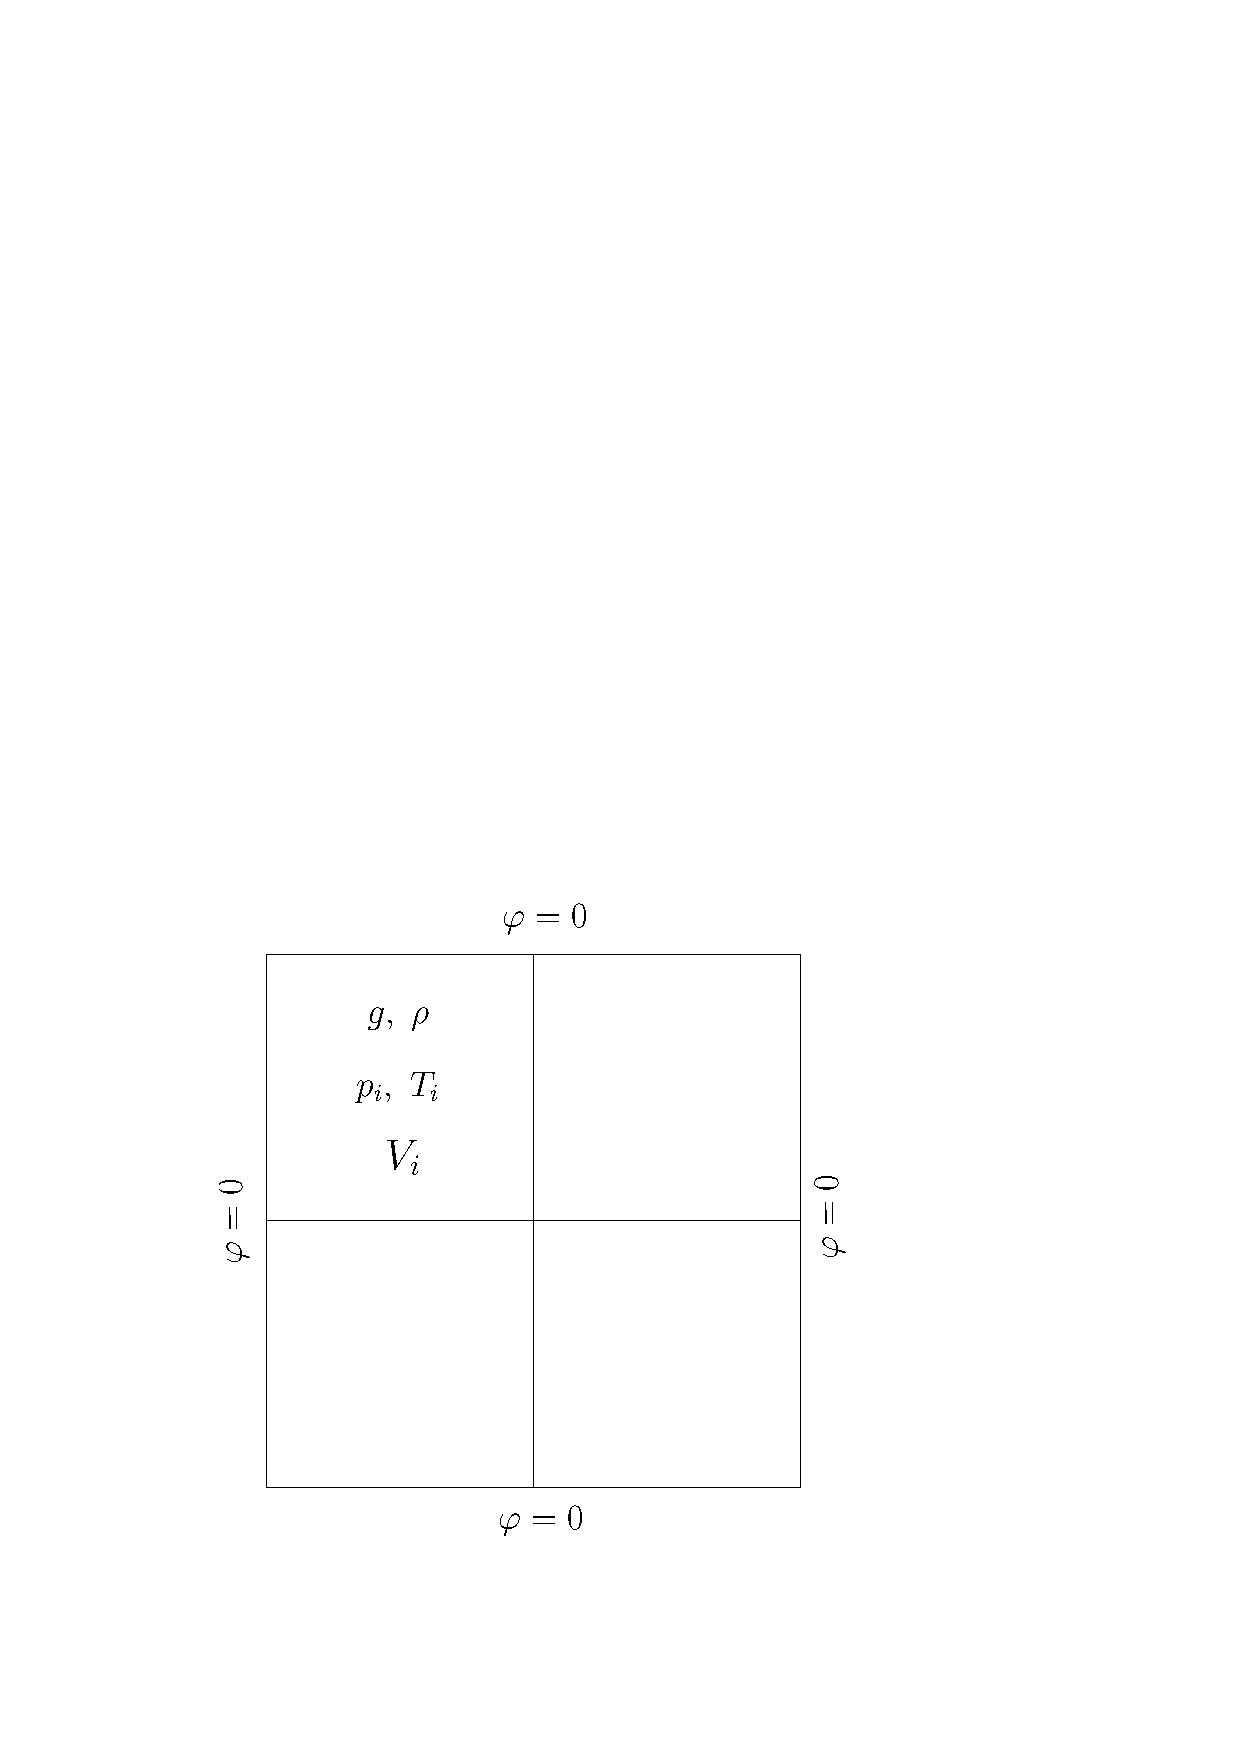
\includegraphics[scale=0.6]{geometry}
	\label{fig:geometry}
\end{center}
As a first example, we may assume that $T$ and $p$ are constant in each patch and $\rho$ is uniform over the whole membrane. We will be interested in the following global quantities:
\begin{itemize}
	\item $\displaystyle\int_V\varphi(x,y)\dxy\ \ldots$ \parbox[t]{7.5cm}{total volume of fluid contained in the flipped canopy formed by the deflected membrane,}
	\item $\displaystyle\int_{V_i}\varphi(x,y)\dxy\ \ldots$ \parbox[t]{7.5cm}{total volume of the fluid column above patch $V_i$.}
\end{itemize}
\end{document}
